\documentclass[11pt,letterpaper]{article}
%\documentclass[11pt,a4paper]{report}

\usepackage{amssymb,amsmath,amsthm} 
\usepackage[margin=2cm]{geometry}
\usepackage{fancyhdr}
\usepackage{enumitem}
\usepackage[compact]{titlesec}
\usepackage{graphicx,ctable,booktabs,subfigure}

\usepackage{xparse,hyperref,parskip}

%\newcommand{\abs}[1]{\left|#1\right|}

\newcommand{\semester}{Spring 2022}
\newcommand{\due}{Tuesday, February 8}


\pagestyle{fancy}
\lhead{ }
\chead{\footnotesize Math 3338\quad  Numerical Methods\quad  \semester}
\rhead{\footnotesize \thepage}
\setlength{\parindent}{0cm}
\setlist{noitemsep}



\input{defs.tex}

%Defines the problem environment with arguments Points and Solution gap
\input{problem_env.tex}



\begin{document}

\begin{center}
{\huge{\bf  Numerical Methods}} \\[1.5ex]
{\bf Math 3338 -- \semester}\\[1.5ex]
{\Large{\bf Worksheet 7\ \\[2ex] Integration Errors}}\\
\end{center}
\vspace{2mm}

\section{Reading}

\begin{table}[!ht]
 \centering
 \begin{tabular}{ll}
   CP & 5.2, 5.3, 5.4 \\
 NMEP & 6.3
 \end{tabular}
\caption{Sections Covered}
\end{table}



\section{Error}
We know how to calculate integrals for a set number of steps. However, we typically care far 
more about accuracy. We know that more more steps will produce more accuracy, but we also
don't want our computer to run forever. 

%\subsection{Estimating Error}
We're going to focus on the trapezoidal method, there are similar rules for Simpson's method but 
they aren't really necessary. We're also going to concentrate on a method that doesn't require
that we know the explicit function being integrated. This is useful as we typically don't know
the function. If we have data given by an experiment, it may just give a sequence of points.


Suppose we use $N_1$ subintervals to get an approximate area of $I_1$. The width of each 
subinterval is $h_1=\frac{b-a}{N_1}$. The trapezoidal method gives an error $O(h_1^2)$ (the book
proves this), if $I$ is the actual area, then
\[
I = I_1+O(h_1^2) = I_1+ch_1^2
\]
where $c$ is some constant. Double the number of steps, $N_2=2N_1$ say the area is $I_2$. Now,
our width is $h_2=\frac{1}{2}h_1$ and the area is
\[
 I = I_2+O(h_2^2) = I_2+ch_2^2
\]
Set these two equations equal, the error is $I_2-I_1$,
\[
I_2-I_1 = ch_1^2-ch_2^2 = 3ch_2^2
\]
In reality, the error is $\epsilon = ch_2^2$, so
\[
\epsilon = \frac{1}{3}(I_2-I_1)
\]

This is useful! If we want our area to be accurate up to 4 decimals, we keep doubling the 
number of subintervals until $\epsilon<.0001$.

The naive thing to do would be to set up a loop and continually double the number of steps until
until you get an acceptable error. This is naive because you'll be repeating computations, you'd
have to compute $f(a)$ every single time. 
\begin{figure}[!ht]
 \centering
 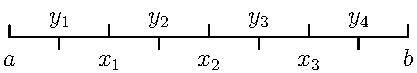
\includegraphics{images/interval.pdf}
 \caption{Breaking an interval}
 \label{fig:interval}
\end{figure}
It's more efficient if each time you double the number of intevals, you only add the new steps.
For example, in Figure \ref{fig:interval} there are initially 4 subintervals, denoted under the 
axis. Doubling this to 8 adds the $y$'s above the axis. The trapezoid method for the 8 intervals
would be similar to,
\[
\frac{1}{2}f(a)+\frac{1}{2}f(b) + \sum_{i=1}^3 f(x_i) + \sum_{i=1}^4 f(y_i).
\]
Notice the first three terms are the trapezoid rule for 4 intervals. Note that it's not exactly
this. Figure it out.


\section{Romberg Integration}
If our goal is to minimize error, it seems counter intuitive to rely on the trapezoid method. We've
already seen Simpson's rule leads to a better approximation. What if there was a way to extend the
trapezoid rule to be more precise than Simpson's rule, while simultaneously being easier to code?

First, using Talyor series we could show the error of the trapezoid method is,
\begin{equation}
 I = I_i + c_1h_i^2 + c_2h_i^4 + c_3h_i^6+\cdots
\label{eqn:traperr}
\end{equation}
Where $I_i$ is the approximation using steps with width $h_i$. If we want a certain approximation
error, we truncate the summation. So $I = I_i+c_1h_i^2$ is accurate to $O(h_i^4)$. Similar to 
what we did before, let's say $h_{i-1} = 2h_i$, then the $(i-1)$-approximation is
\begin{align}
 I = & I_{i-1}+c_1h_{i-1}^2 + c_2h_{i-1}^4 + \cdots \nonumber\\
   =  & I_{i-1} + 2^2 c_1h_i^2 + 2^4c_2h_i^4+\cdots \label{eqn:trapsmall}
\end{align}

Equations (\ref{eqn:traperr}) and (\ref{eqn:trapsmall}) are equal. Truncate after the $h_i^2$ term
and subtract to find,
\begin{equation*}
 0 = (I_i-I_{i-1}) - (2^2-1)c_1h_i^2
\end{equation*}
Solve this for $c_1h_i^2$ to find,
\[
 c_1h_i^2 = \frac{1}{4^1-1}(I_i-I_{i-1}).
\]
Then
\begin{align*}
I = & I_i +\frac{1}{4^1-1}(I_i-I_{i-1}) + c_2h_i^4 + c_3h_i^6+\cdots \\
  = & R_{i,2} + c_2h_i^4+\cdots
\end{align*}
is accurate to order 4. Notice we've used the variable $R_{i,2} = I_i + \frac{1}{4^1-1}(I_i-I_{i-1})$. This is essentially a free computation, as we would have calculated them
anyway. 

This is the core of Romberg integration. The general formula is,
\begin{align*}
R_{i,1} = I_i && R_{i,m} = R_{i,m-1} + \frac{1}{4^{m-1}-1}(R_{i,m-1}-R_{i-1,m-1}).
\end{align*}
Where $I_i$ is the result of trapezoidal integration with $2^i$ subintervals. The derivation of this is inductive. Suppose we know $R_{i,k}$ for all $i\le n$ and $1<k\le m$,
then
\begin{equation*}
I = R_{i,m} + c_m h_i^{2m} = R_{i-1,m} + 2^{2m}c_mh_i^{2m}
\end{equation*}
Solve for $c_mh_i^{2m}$ to find,
\[
 c_mh^{2m} = \frac{1}{4^m-1}(R_{i,m}-R_{i-1,m})
\]
which gives the Romberg recursion formula.

\newpage

\begin{center}
{\huge{\bf  Numerical Methods}} \\[1.5ex]
{\bf Math 3338 -- \semester}\\[1.5ex]
{\Large{\bf Homework 7 (Due: \due)}}\\
\end{center}
\vspace{2mm}



\begin{problem}
 Write two functions that evaluate the trapezoid to a desired degree of accuracy. The inputs
to both will be the same, $f$, $a$, $b$, and $tol$ which should default to $1e-6$, or $10^{-6}$. 
This is the tolerance, and your answer should be at least that accurate. Both functions should return
an answer of the form \texttt{(approximation, number of steps)}.

Call the first function \texttt{trap\_naive}. This function should use your old \texttt{trapezoid}
method to compute each approximation. 

Call the second \texttt{trap\_error}. For this function you should be clever and only compute the
new steps at each iteration.

Evaluate $\int_0^1 \sin^2(\sqrt{100x})\,dx$ for several small tolerances 
$tol\in\{10^i\vert -13\le i\le -1\}$. Make a table that contains the tolerance, the number of steps, 
and time for both methods. Discuss  your observations. 
\end{problem}


\begin{problem}
Write a function called \texttt{romberg}. The inputs are $f$, $a$, $b$, and $tol$ which should 
default to $1e-6$, or $10^{-6}$. This is the tolerance, and your answer should be at least that 
accurate. Both functions should return an answer of the form \texttt{(approximation, number of steps)}.

Evaluate $\int_0^1 \sin^2(\sqrt{100x})\,dx$ for several small tolerances 
$tol\in\{10^i\vert -13\le i\le -1\}$. Make a table that contains the tolerance, number of steps
and time for both \texttt{romberg} and \texttt{trap\_error}.

Compare and discuss.
\end{problem}



\begin{problem}
Many of these methods already exist. Let's compare ours to the pre-built ones. Here is a help page
\url{https://docs.scipy.org/doc/scipy-0.14.0/reference/integrate.html}. This is part of the
scipy package. Put the following at the top of your file \texttt{from scipy import integrate}, now
we have access to the integrate package.

Make a table that compares the run time of \texttt{romberg}, \texttt{integrate.romberg} and 
\texttt{integrate.quadrature}. To set the tolerance you'll need to use the keyword \texttt{tol}
in the later two. Do this for $tol\in\{10^i\vert -13\le i\le -1\}$.

Compare and discuss the run times for each. Note that I noticed something strange with the quadrature
times, if something similar happens on yours, you should mention it.

\end{problem}




\end{document}




































